\documentclass[border=6pt]{standalone}
\usepackage[edges]{forest}
\usetikzlibrary{arrows.meta}
\begin{document}
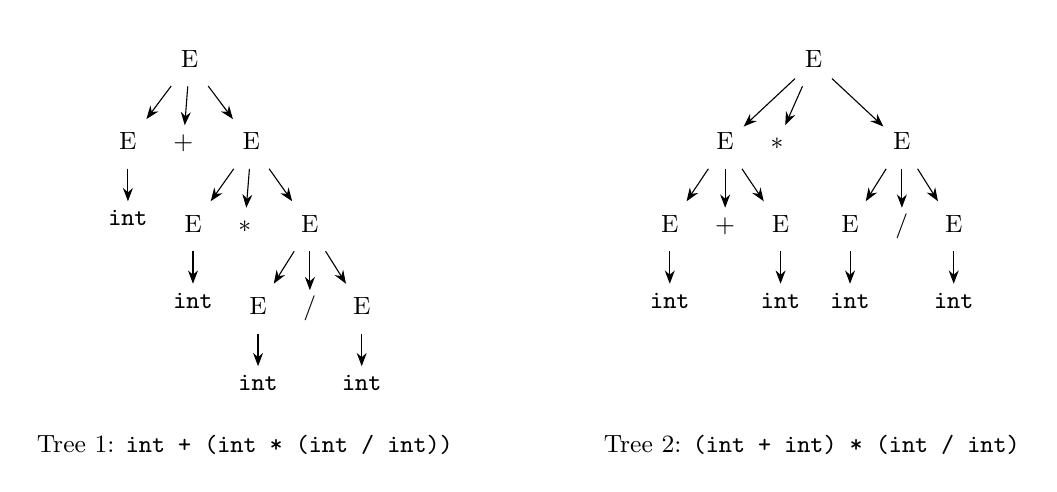
\begin{tikzpicture}
\node[anchor=north] at (0,0) {\begin{forest}
for tree={align=center,font=\small,l=0.7cm,s sep=3mm,edge={->,>=Stealth}},
tm/.style={font=\ttfamily\small,inner sep=1pt},
[E
  [E [int,tm]]
  [{$+$},tm]
  [E
    [E [int,tm]]
    [{$*$},tm]
    [E
      [E [int,tm]]
      [{$/$},tm]
      [E [int,tm]]
    ]
  ]
]
\end{forest}};
\node[font=\small] at (0,-5.3) {Tree 1: \texttt{int + (int * (int / int))}};
\node[anchor=north] at (7.2,0) {\begin{forest}
for tree={align=center,font=\small,l=0.7cm,s sep=3mm,edge={->,>=Stealth}},
tm/.style={font=\ttfamily\small,inner sep=1pt},
[E
  [E
    [E [int,tm]]
    [{$+$},tm]
    [E [int,tm]]
  ]
  [{$*$},tm]
  [E
    [E [int,tm]]
    [{$/$},tm]
    [E [int,tm]]
  ]
]
\end{forest}};
\node[font=\small] at (7.2,-5.3) {Tree 2: \texttt{(int + int) * (int / int)}};
\end{tikzpicture}
\end{document}
